% % Macros.tex

%%%%%%%%%%%%%%%%% Definition of commands

%\newtheorem{theorem}{Theorem}{}
%\newtheorem{lemma}[theorem]{Lemma}{}

\newtheorem{theorem}{Theorem}{}
\newtheorem{definition}{Definition}{}
\newtheorem{proposition}{Proposition}{}
\newtheorem{corollary}{Corollary}{}
\newtheorem{example}{Example}{}
\newtheorem{lemma}{Lemma}{}
\long\def\BEGINOMIT#1\ENDOMIT{\relax}  % to omit large portions of text

\def\adwin{{\tt ADWIN }}
%\def\adwintwo{{\tt ADWIN2 }}
\def\adwindt{AHTree }
\def\adwinb{{\tt ADWIN}}
%\def\adwintwob{{\tt ADWIN2}}
\def\adwindtb{AHTree}
\def\hwt{HWTree}
\def\HWTAdwin{HWT-\adwin }
\def\HWTAdwinb{HWT-\adwinb}
\def\HWTsAdwin{$\mbox{HWT}^*$\adwin }
\def\HWTsAdwinb{$\mbox{HWT}^*$\adwinb}
\def\HATAdwin{HAT-\adwin }
\def\HATAdwinb{HAT-\adwinb}

\def\Section{\section}

\def\sizeGraph{0.42}
%\newenvironment{proof}{Proof.}{\square\\}
\def\square{\hfill\nobreak\rule{1ex}{1.4ex}}
\def\abovespace{\vspace{.05cm}}
\def\belowspace{\vspace{.05cm}}


\def\hmu{\hat{\mu}}
\def\eps{\epsilon}
\def\epsc{\epsilon_{cut}}
\def\hmuu{\hat{\mu}_{W_1}}
\def\hmuz{\hat{\mu}_{W_0}}
\def\muu{{\mu}_{W_1}}
\def\muz{{\mu}_{W_0}}
%\def\change{\bf}
\def\change{}


\long\def\BEGINOMIT#1\ENDOMIT{\relax}  % to omit large portions of text
\def\TreeNat{{\sc TreeNat}}
\newcommand{\head}{\textsf{head}}
\newcommand{\tail}{\textsf{tail}}
\newcommand{\fc}[1]{\begin{center}\epsfig{file=#1}\end{center}}
\def\tq{\bigm|}
\def\implies{\Rightarrow}
\def\supp{\hbox{\rm supp}}
\def\qed{\hfill $\Box$}





%%%%%%%%%%%%%%%%%%%%%%%%%%%%%%%%%%%%%%%%%%%%%%%%%%%%%%%


%%%%%%%%%%%%%%%%% Definition of commands from the Berlin workshop

\newcommand{\onenode}{\begin{picture}(5,5) \put(3,3){\circle*{3}}
\end{picture} }
%\newcommand{\twonodes}{\begin{picture}(5,18)
%\put(3,3){\circle*{3}}\put(3,3){\line(0,1){12}}\put(3,15){\circle*{3}}
%\end{picture}}
\newcommand{\twonodes}{\begin{picture}(12,5) \put(3,3)
{\circle*{3}}\put(3,3){\line(1,0){6}}\put(9,3){\circle*{3}}
\end{picture}}
%\newcommand{\fdem}{\hfill$\Box$}

\def\tq{\bigm|}
\def\implies{\Rightarrow}
\def\supp{\hbox{\rm supp}}
\def\qed{\hfill $\Box$}

\def\C{{\Delta}}
\def\D{{\cal D}}
\def\U{{\cal U}}
\def\H{{\cal H}}
\def\R{{\cal R}}
\def\V{{\cal V}}
\def\M{{\cal M}}
\def\I{{\cal I}}
\def\implies{\rightarrow}
\def\st{\bigm|}


%\input{TreeMacros}
%%%%%%%%%%%%%%%%%%%%%%%%%%%%%%%%%%%%%%%%%%%%%%%%%%%%%%%%%
% Tree definitions
\def\Ts#1#2{
\node at (#1,#2) {}
child {
	node {}
}
child {
	node {}
	child {
		node {} 	
		child {node {}} 
	}
	child {node {}}
}; 
}
\def\Tsa#1#2{
\node (a) at (#1,#2) {D}
child {
	node {B}
	child {
		node {C} 	
		child {node {A}} 
	}
	child {node {C}}
}; 
}
\def\Tsb#1#2{
\node (b) at (#1,#2) {D}
child {
	node {B}
	child {
		node {C} 	
	}
	child {node {C}}
}
child {
	node {B}
}; 
}
\def\Tsc#1#2{
\node (c) at (#1,#2) {D}
child {
	node {B}
	child {
		node {C} 
		child {node {A}}	
	}	
}
child {
	node {B}
}; 
}
\def\Tsbc#1#2{
\node (bc) at (#1,#2) {D}
child {
	node {B}
	child {
		node {C} 
	}	
}
child {
	node {B}
}; 
}
\def\Tsab#1#2{
\node (ab) at (#1,#2) {D}
child {
	node {B}
	child {	node {C} }
	child {node {C}}
}; 
}
\def\Tsac#1#2{
\node (ac) at (#1,#2) {D}
child {
	node {B}
	child {
		node {C} 	
		child {node {A}} 
	}
}; 
}
\def\Tsabc#1#2{
\node (abc) at (#1,#2) {D}
child {
	node {B}
	child {	node {C} }
}; 
}
\def\Tsd#1#2{
\node (d) at (#1,#2) {D}
child {	node {B}	}
child {	node {B}}; 
}

\def\Tsdd#1#2{
\node (d) at (#1,#2) {D}
child {	node {B}	}
; 
}

\def\Tsx#1#2{
\node (c) at (#1,#2) {}
child {
	node {}
	child {
		node {} 
		child {node {}}	
	}	
}
child {
	node {}
	child {	node {}}
	child {	node {}} 
}; 
}


\def\Tse{
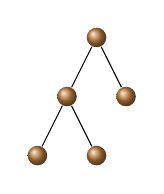
\begin{tikzpicture}[scale=.5, auto,swap, inner sep=2.5pt,]% scale=1, inner sep=5
%\useasboundingbox
%\tikz[baseline]
\tikzstyle{every node}=[ball color=brown,circle,text=white]%, minimum size=2mm]
\node at (5,0) {}
child {
	node {} 
	child {node {}}
	child {
		node {} 	
		%child {node {}} 
	}	
}
child {node {}};

;

%\begin{scope}
%\tikzstyle{every node}=[]
%\draw(2,-2) node {$\longrightarrow$};
%\end{scope}

\end{tikzpicture}
}
%%%%%%%%%%%%%%%%%%%%%%%%%%%%%%%%%%%%%%%%%%%%%%%%%%%%%%%%%
% Slide explaining NOT IMPLICIT rule
\def\Treex{

\begin{center}
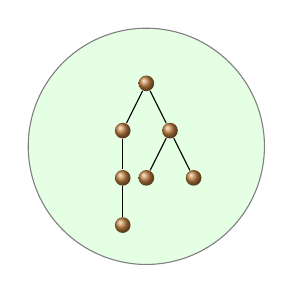
\begin{tikzpicture}[scale=.4, auto,swap, inner sep=2pt,]% scale=1, inner sep=5
%\useasboundingbox
%\tikz[baseline]

\tikzstyle{every node}=[draw=black!50,fill=green!10]
\node (ta) at (8,-2) [circle,inner sep=0pt,minimum width=3cm,minimum height=3cm] {};
%,pin=below:{\textbf{Supertree} of the antecedents} 
%pin=-120:NO Supertree of the consequent

\tikzstyle{every node}=[ball color=brown,circle,text=white]
\Tsx{8}{0}

\end{tikzpicture}

\vspace{.5cm}

This supertree of the antecedents %} supertree
is \textbf{NOT} a supertree of the consequents.% supertree 

\end{center}

}

\def\DataSet{
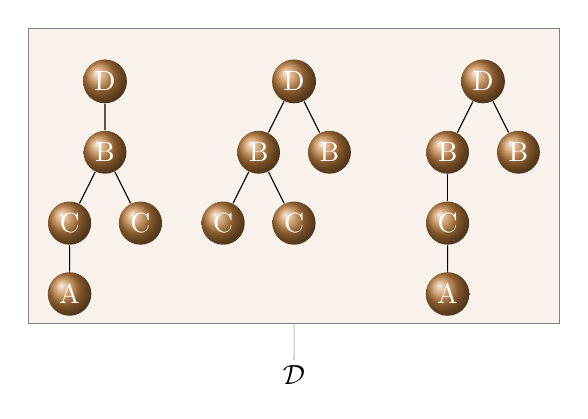
\begin{tikzpicture}[scale=.6, auto,swap, inner sep=2pt,]% scale=1, inner sep=5
%\useasboundingbox
%\tikz[baseline]

\tikzstyle{every node}=[draw=black!50,fill=brown!10]
\node (ta) at (8,-2) [rectangle,inner sep=0pt,minimum width=6.75cm,minimum height=3.75cm,pin=below:${\cal D}$] {};


\tikzstyle{every node}=[ball color=brown,circle,text=white]%, minimum size=1mm]

 \Tsa{4}{0};
 \Tsb{8}{0};
 \Tsc{12}{0};

\end{tikzpicture}
}

%%%%%%%%%%%%%%%%%%%%%%%%%%%%%%%%%%%%%%%%%%%%%%%%%%%%%%%%%
% Lattices
\def\Lattice{

\begin{tikzpicture}[scale=.6, auto,swap, inner sep=2pt,]% scale=1, inner sep=5
%\useasboundingbox
%\tikz[baseline]
\LatticeAux
\end{tikzpicture}
}

\def\LatticeAux{
\tikzstyle{every node}=[ball color=brown,circle,text=white]%, minimum size=2mm]

 \Tsa{5}{0};
 \Tsb{10}{0};
 \Tsc{15}{0};

 \Tsab{5}{-7};
 \Tsac{10}{-7};
 \Tsbc{15}{-7};

 \Tsabc{10}{-14};

\tikzstyle{every node}=[draw=black!50]%fill=blue!20,minimum size=5mm]%, minimum size=2mm]
  %\draw[style=help lines] (-1,-2) grid (6,3);

%\tikzstyle{place}=[circle,draw=blue!50,fill=blue!20,thick,
%                   inner sep=0pt,minimum size=6mm]

\node (ta) at (5,-2.5) [ellipse,inner sep=0pt,minimum width=2.25cm,minimum height=3.75cm,label=-120:$1$] {};
\node (tb) at (10,-2) [ellipse,inner sep=0pt,minimum width=3cm,minimum height=3cm,label=below:$2$] {};
\node (tc) at (15,-2.5) [ellipse,inner sep=0pt,minimum width=2.25cm,minimum height=3.75cm,label=-60:$3$] {};

\node (tab) at (5,-9) [ellipse,inner sep=0pt,minimum width=2.25cm,minimum height=3cm,label=-120:$1 2$] {};
\node (tac) at (10,-9) [ellipse,inner sep=0pt,minimum width=2.25cm,minimum height=3.75cm,label=-60:$1 3$] {};
\node (tbc) at (15,-9) [ellipse,inner sep=0pt,minimum width=2.25cm,minimum height=3cm,label=-60:$2 3$] {};

\node (tabc) at (10,-15.7) [ellipse,inner sep=0pt,minimum width=2.25cm,minimum height=3cm,label=below:$1 2 3$] {};

  %\path (0,0) node(aa) [rectangle,draw,minimum size=1cm]     {}
  %      (5,0) node(b) [circle,draw]               {}
  %      (10,-7) node(c) [rectangle,draw] {}
  %      (10,-14) node(d) [rectangle,draw] {};
  \draw[thick,blue!50] (ta) -- (tab) -- (tabc) -- (tbc) -- (tc) -- (tac) -- (tabc) -- (tab) -- (tb)
	 -- (tbc);
   \draw[thick,blue!50] (ta) -- (tac);
  %\draw[thick,red,->] (a) |- +(1,3) -| (c) |- (b);
  %\draw[thick,blue,<->] (b) .. controls +(right:2cm) and +(down:1cm) .. (d);
}


